
\documentclass[a4paper]{article}
\usepackage[utf8]{inputenc}

\usepackage[english,german]{babel} 
\usepackage[utf8]{inputenc}

\usepackage{alltt}
\usepackage{amsmath}
\usepackage{amssymb}
\usepackage{amsthm}
\usepackage{color}
\usepackage{enumitem}
\usepackage{epsfig}
\usepackage{fancyhdr}
\usepackage{float}
\usepackage{framed}
\usepackage{graphicx} 
\usepackage{graphics}
\usepackage{hyperref}
\usepackage{listings}
\usepackage{multirow}
\usepackage{tabularx}
\usepackage{textcomp}
\usepackage{tikz}
\usepackage{url}
\usepackage{vmargin}
\usepackage{xspace}
\usepackage{comment}
\usetikzlibrary{calc,trees,positioning,arrows,chains,shapes.geometric,%
    decorations.pathreplacing,decorations.pathmorphing,shapes,%
    matrix,shapes.symbols,topaths,matrix}
\newcommand{\question}[2][0]{\section{{#2} \hfill ({#1} P.)}}
\setpapersize{A4}
\setmargins{2.5cm}{2.0cm}% % linker & oberer Rand
         {16cm}{22cm}%   % Textbreite und -hoehe
           {48pt}{36pt}%   % Kopfzeilenhoehe und -abstand
           {0pt}{30pt}%    % \footheight (egal) und Fusszeilenabstand

\frenchspacing
\pagestyle{fancy}
\sloppy

\newcommand{\hide}[1]{}

\markright{Kopfzeile}


\tikzset{
>=stealth',
  punktchain/.style={
    rectangle,
    rounded corners,
    % fill=black!10,
    draw=black, very thick,
    text width=10em,
    minimum height=3em,
    text centered,
    on chain},
  line/.style={draw, thick, <-},
  element/.style={
    tape,
    top color=white,
    bottom color=blue!50!black!60!,
    minimum width=8em,
    draw=blue!40!black!90, very thick,
    text width=10em,
    minimum height=3.5em,
    text centered,
    on chain},
  every join/.style={->, thick,shorten >=1pt},
  decoration={brace},
  tuborg/.style={decorate},
  tubnode/.style={midway, right=2pt},
}


\setlength{\parindent}{0pt}
\setlength{\parskip}{5pt}
\fboxsep1.5mm


\lstdefinestyle{mystyle}{
    backgroundcolor=\color{white},   
    commentstyle=\color{codegray},
    keywordstyle=\bf \ttfamily \color{codepurple},
    numberstyle=\tiny\color{codegray},
    stringstyle=\color{codegreen},
    basicstyle=\footnotesize,
    breakatwhitespace=false,         
    breaklines=true,                 
    captionpos=b,                    
    keepspaces=true,                 
    numbers=left,                    
    numbersep=5pt,                  
    showspaces=false,                
    showstringspaces=false,
    showtabs=false,                  
    tabsize=8,
    keepspaces,
    extendedchars=true, 
      upquote=true,
    columns=fixed,
    showstringspaces=false,
    extendedchars=true,
    breaklines=true,
    frame=single,
    showspaces=false,
    showstringspaces=false,
    rulecolor=\color{white},
}

\lstdefinelanguage{sql}[]{}{
        %tag=[s]<>,      % =*: also apply styles within tag, =**: cumulate styles
        morekeywords={sql, VIEW, AS, FROM, SELECT, WHERE, FUNCTION, BOOLEAN, RETURNS, DETERMINISTIC, RETURN, REFERENCES, WITH, SEQUENCE, TRUNCATE, START, CREATE, AS, LANGUAGE, FUNCTION, CURSOR, PREPARE, OPEN, USING, CLOSE, DECLARE, END, BEGIN, EXEC, SQL, CONNECT TO, DISCONNECT, COMMIT, LOOP, IF, THEN, ELSE, WHILE, BREAK, EXIT, INSERT, INTO, VALUES, UPDATE, SET, TABLE, PRIMARY, KEY, AND, UNION, ALL, JOIN, ON, GROUP, BY, MATERIALIZED, INT, DATE, COUNT, ORDER, OVER, PARTITION, ASC, DESC, VARCHAR, NOT, NULL, PRIMARY, KEY, DECIMAL, SUM, AVG, ROWS, BETWEEN, PRECEDING, CURRENT, ROW, INSTEAD, TRIGGER, OF, FOR, EACH, EXECUTE, PROCEDURE, DISTINCT, HAVING, LIMIT},
morestring=[s]{'}{'},
morecomment=[l]{--}
        %sensitive=false
}

\lstset{style=mystyle,numbers=none,basicstyle=\ttfamily,upquote=true}

 
\definecolor{codegreen}{rgb}{0,0.6,0}
\definecolor{codegray}{rgb}{0.5,0.5,0.5}
\definecolor{codepurple}{rgb}{0.38,0,0.72}
\definecolor{backcolour}{rgb}{0.95,0.95,0.92}
\definecolor{backcolourSingleCode}{rgb}{0.95,0.95,0.92}

\newcommand{\subtitle}{\textbf{Exercise 9}}
\newcommand{\outdate}{08.01.2024}
\newcommand{\duedate}{15.01.2024 12:00 MEZ}
\newcommand{\video}{049}

\begin{document}

\lhead{\begin{tabular}{l}
{\bf Database Systems WS 2023/24}\\
{\bf \subtitle: Distributed \outdate, Due \duedate}\\
{Submitted by }
\end{tabular}
}
\rhead{}

\question[1]{Skyline Queries}

Given the TPC-H\footnote{\url{http://dbis.informatik.uni-kl.de/files/teaching/ws1819/dbs/protected/tpch.dmp.gz}} table \textbf{''part''}.

We want to compute the skyline over the following four dimensions:
\begin{itemize}
\item \emph{p\_size:} larger is better,
\item \emph{p\_retailprice:} less is better,
\item \emph{p\_container:} Use the function \texttt{getContainerSize} from below: less is better.
\item \emph{p\_brand:} Cannot be compared.
\end{itemize}

In OLAT you will find a file \texttt{skylineFunc.sql}, which implements the \texttt{getContainerSize} function.
You can either copy the create-statement from the file and execute it in your DBMS or you can directly execute the file with the following command (you may have to change the database name to the one you used to create it).
\begin{verbatim}
psql -d tpch -f skylineFunc.sql
\end{verbatim} 

\begin{enumerate}
\item Create a SQL query to calculate the number of elements in the skyline defined above (without using the \verb+SKYLINE+-operator).
Submit the query and the result.\\\\
{\bf Solution:}\\
\begin{lstlisting}[language=sql]
SELECT COUNT(*) 
FROM part p
WHERE NOT EXISTS(
SELECT *
FROM part p1
WHERE p1.p_size >= p.p_size
AND p1.p_retailprice <= p.p_retailprice
AND getContainerSize(p1.p_container) <= getContainerSize(p.p_container)
AND p1.p_brand = p.p_brand
AND (p1.p_size > p.p_size OR p1.p_retailprice < p.p_retailprice OR getContainerSize(p1.p_container) < getContainerSize(p.p_container)))
\end{lstlisting}

The output of the query is 250.


\item Write the same query using the \verb+SKYLINE+-operator. (You do not have to install the plugin and execute the query.)\\\\
{\bf Solution:}\\
\begin{lstlisting}[language=sql]
SELECT COUNT(*) 
FROM part p
SKYLINE OF p.p_size MAX, p.p_retailprice MIN, 
  getContainerSize(p.p_container) MIN, p.p_brand DIFF;
\end{lstlisting}

\end{enumerate}

\question[1]{Skyline NN}

Implement the nearest neighbor (NN) method to compute skylines in a language of your choice. A basic Java template is available in OLAT.
This template provides a (fake) R-Tree implementation which can be used to query for the nearest neighbor of a point, all points within a rectangle, and the nearest neighbor within a rectangle.
If you are using another language, you are allowed to also implement a fake R-Tree with the methods described above (or use a real implementation without a included skyline function).

The program should output the calculated skyline (the template already takes care of this).

Submit your code and the output for the following points (If you use the template, the points are already included):

$$(10,20),(12,10),(8,11),(16,19),(6,4),(5,6),(14,12),(2,5),(3,10),(13,19),(17,5),(9,3),(20,8),(8,10)$$
\\\\
{\bf Solution:}\\
\begin{figure}[H]
  \centering
  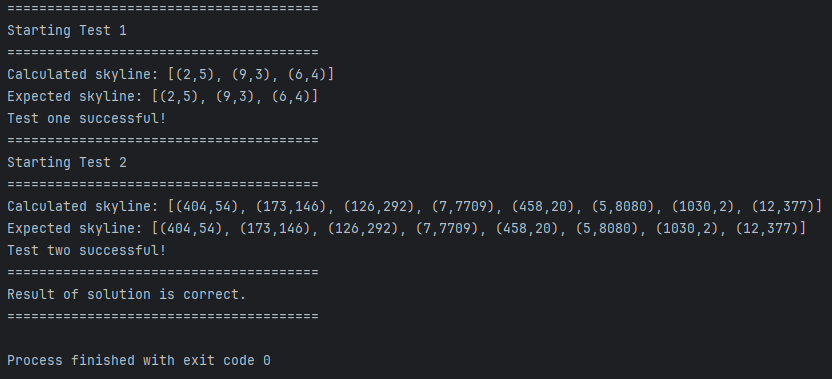
\includegraphics[scale = 0.6]{SkylineOutput.png}
\end{figure}

\newpage

\question[1]{Transactions}

\begin{enumerate}
	\item \textbf{A database has the consistency condition $0\leq A\leq B$. Describe, for the following transactions, if the condition is fulfilled. Explain your answer.}

    \begin{enumerate}

    \item[$T_1: $] \quad {\tt B:= 2*A; A:= 2*B;}
    \item[$T_2: $] \quad {\tt B:= A+1; A:= B+1;}
    \item[$T_3: $] \quad {\tt A:= A+2*B; B:= 2*A+B;}
    \end{enumerate}

\textbf{Solution}: The consistency condition of database is met \textbf{if $0\leq A\leq B$}. 

\begin{enumerate}

  \item[$T_1: $] \quad {\tt B:= 2*A; A:= 2*B;}
  
  Here, B is updated before A. Hence, the value of B upon solving would become
  \[B:= 2*A ; \textbf{B:= 2A}\]
  When A gets updated, it would fetch the value of B from the previous output to process the transaction
  \[A:= 2*B ; A:= 2*2A ; \textbf{A:=4A}\]

  The value of A is greater than the value of B. Hence, the \textbf{\color{red} database consistency condition is not met} in this case.

  Let us consider the values of A = 1 and B = 1 for the given transaction, then the value of B would be  \[B:= 2A ; \textbf{B:= 2}\]
  The value of A would be \[A:=4A; \textbf{A:= 4}\]. Even in this case, \textbf{\color{red}the database consistency condition is not met.}

  Let us consider the values of A = 0 and B = 0 for the given transaction, then the value of B would be  \[B:= 2A ; \textbf{B:= 0}\] 
  The value of A would be \[A:=4A; \textbf{A:= 0}\] In this case, \textbf{\color{blue}the database consistency condition is met when A:= 0 and B:= 0};

  
  \item[$T_2: $] \quad {\tt B:= A+1; A:= B+1;}

  Here also the database consistency condition is not met because B is updated before A and later it is being using while processing.
  The value of \textbf{B:= A+1;} 
  
  The value of A would be $A:= B+1; A:= A+1+1;$ (Substituted the value of B from previous output)
  \textbf{A:= A+2;}

  Considering the values of A=1 and B=1 and substituting in the above equations we get,
  
  \textbf{B:=2 ; A:=3} -(i)
  
  Even if we consider the values of A=0 and B=0, we get \textbf{B:= 1 ; A:=2} -(ii)

  In both the cases (i) and (ii), A is greater than B, \textbf{\color{red}the database consistency condition is not met.}
  
  \item[$T_3: $] \quad {\tt A:= A+2*B; B:= 2*A+B;}
  
  Here, A got updated before B and later the value of A was used in B, there might be chances that the database consistency condition is met.
  
  Solving the values of A and B, we get
  
  \textbf{A:= A+2*B} and
  
  B:= 2*A+B; B:= 2*(A+2*B)+B (Substituting the value of A from above) 
  
  \textbf{B:= 2A+5B}

  Let us consider the values of A = 1 and B = 1 for the given transaction. Substituting the value of A and B in A:= A+2*B; we get \textbf{A:=3} -(iii)
 
  Substituting the value of A (by considering the previous output of A) and B in B:= 2A+5B; we get \textbf{B:=11} -(iv)

  Let us consider the values of A = 0 and B = 0 for the given transaction. Substituting the value of A and B in A:= A+2*B; we get \textbf{A:=0} -(v)
  
  Substituting the value of A (by considering the previous output of A) and B in B:= 2A+5B; we get \textbf{B:=5} -(vi)

  Hence from (iii), (iv), (v) and (vi), we can say that, $A \leq B$ and the \textbf{\color{blue}database consistency condition is met.}



  \end{enumerate}



\item \textbf{For each of the previous transactions, provide the input, read, and write operations. Assume immediate write-back of the changed values. Describe the effect of these operations on the main memory and the hard disk. The initial values are $A=5$ and $B=10$.}

\textbf{Solution}: Input loads the data from Disk to Main memory, Read and Write operations are performed in transactions local address space, Output loads the data from Main memory back to Disk.

$T_1: $ \quad {\tt B:= 2*A; A:= 2*B;}

  \textbf{INPUT(A)} : Loads A from Disk to Main memory (A=5)\\
  \textbf{READ(A,t)}: Reads the value of A from Main memory to the local transaction variable \\
  \textbf{t:= 2 * A}: Computes the value of A (t:= 2*5= 10)\\
  \textbf{WRITE(B,t)}: Immediate write-back of changed values. Writes the value of B from local transaction variable to Main memory \textbf{(B:= 10)}\\
  \textbf{READ(B,t)}: Reads the value of B from the Main memory \\
  \textbf{t:= 2 * B}: Computes the value of B (t:=2 * 10 = 20)\\
  \textbf{WRITE(A,t)}: Writes the value of A from local transaction variable to Main memory \textbf{(A:= 20)}\\
  As per database consistency condition, $A \leq B$ but $T_1$, $A > B$ which does not meet the condition.\\
 
$T_2: $ \quad {\tt B:= A+1; A:= B+1;}

  \textbf{INPUT(A)} : If A is not present in Main memory, it gets loaded from Disk (A=5)\\
  \textbf{READ(A,t)}: Reads the value of A from Main memory to the local transaction variable \\
  \textbf{t:= A + 1}: Computes the value of A (t:= 5 + 1 = 6)\\
  \textbf{WRITE(B,t)}: Immediate write-back of changed values. Writes the value of B from local transaction variable to Main memory \textbf{(B:= 6)}\\
  \textbf{READ(B,t)}: Reads the value of B from the Main memory\\
  \textbf{t:= B + 1}: Computes the value of B (t:=6 + 1 = 7)\\
  \textbf{WRITE(A,t)}: Immediate write-back of changed values. Writes the value of A from local transaction variable to Main memory \textbf{(A:= 7)}\\
  As per database consistency condition, $A \leq B$ but in transaction $T_2$, $A > B$ which does not meet the condition.\\

$T_3: $ \quad {\tt A:= A+2*B; B:= 2*A+B;}

  \textbf{INPUT(A)} : If A is not present in Main memory, it gets loaded from Disk (A=5)\\
  \textbf{READ(A,t)}: Reads the value of A from Main memory to the local transaction variable\\
  \textbf{INPUT(B)} : Loads B from Disk to Main memory (B=10)\\
  \textbf{READ(B,t)}: Reads the value of B from Main memory to local transaction variable\\
  \textbf{t:= A + 2 * B}: Computes the value of A (t:= 5 + 2 * 10 = 25)\\
  \textbf{WRITE(A,t)}: Immediate write-back of changed values. Writes the value of A from local transaction variable to Main memory \textbf{(A:= 25)}\\
  \textbf{READ(A,t)}: Reads the value of A from Main memory to the local transaction variable\\
  \textbf{READ(B,t)}: Reads the value of B from Main memory to local transaction variable\\
  \textbf{t:= 2 * A + B}: Computes the value of B (t:=2 * 25 + 10= 60)\\
  \textbf{WRITE(B,t)}: Immediate write-back of changed values. Writes the value of B from local transaction variable to Main memory \textbf{(B:= 60)}\\

  This transaction $T_3$ satisfies the database consistency condition of  $A \leq B$

  \textbf{OUTPUT} writes the data from Main Memory to Disk upon mentioning after each transaction. Until then, the Main memory would be used. 
  Now that, we did not have to OUTPUT the transactions, the Disk is unaffected.




\item \textbf{Given two transactions $T_1$ and $T_2$ and the following situation (' marks changed entries):}

 \begin{center}

    \begin{tikzpicture}

      \draw (0,0) -- (6,0) -- (6,5.5) -- (0,5.5) -- (0,0);
      \draw (0,1) -- (6,1); \draw (0,2.5) -- (6,2.5); \draw (0,3.5) -- (6,3.5); \draw (0,4.5) -- (6,4.5);
      \draw (2,0) -- (2,1); \draw (4,0) -- (4,1);
      \draw (2,2.5) -- (2,5.5); \draw (4,2.5) -- (4,5.5);
      \node at (3,2) {\dots};

      \node at (10,2.5) [cylinder, shape border rotate=90, draw,minimum height=5cm,minimum width=4cm] {};

      \node at (3,6) {DBMS Buffer, e.g., Main Memory};
      \node at (10,6) {External Memory, e.g., Hard Disk};
      \draw[->] (8,4) -- (6.1,4) node[midway, above] {\footnotesize Insertion};
      \draw[->] (6.1,2) -- (8,2) node[midway, below] {\footnotesize Removal};

      \node at (2.5, 4) {$A^\prime$};
      \node at (3.5, 4) {$D^\prime$};
      \node at (1, 3) {$C^\prime$};
      \node at (3, 0.5) {$B$};

      \draw (9,3.5) -- (11,3.5) -- (11,4.5) -- (9,4.5) -- (9,3.5);
      \node at (8.5,4.5) {$P_A$};
      \node at (9.5,4) {$A^\prime$};
      \node at (10.5,4) {$D$};

      \draw (8.5,2.2) -- (10.5,2.2) -- (10.5,3.2) -- (8.5,3.2) -- (8.5,2.2);
      \node at (8.25,3.2) {$P_C$};
      \node at (9.5,2.7) {$C^\prime$};

      \draw (9.7,0.5) -- (11.7,0.5) -- (11.7,1.5) -- (9.7,1.5) -- (9.7,0.5);
      \node at (9.4,1.4) {$P_B$};
      \node at (10.5,1) {$B$};
    \end{tikzpicture}
  \end{center}
  \vspace{-0.15cm}

  \textbf{The following table describes the operations of $T_1$ and $T_2$ at different times. \\[0mm]}

\vspace{-0.15cm}

\begin{center}
\begin{tabular}{r|rr} 
\multicolumn{1}{r}{Time} & \multicolumn{1}{c}{$T_1$} & \multicolumn{1}{c}{$T_2$} \\ \hline
\multicolumn{3}{c}{} \\
\ 0 & READ(A,a)  & READ(C,c) \\
10  & a:=a+10    & c:=c*2 \\
20  &            & READ(B,b) \\
30  & WRITE(A,a) &  \\
40  & READ(D,d)  & b:=b+c/4 \\
50  & d:=17*d+42 &  \\
60  & OUTPUT(A)  & WRITE(C,c) \\
70  & WRITE(D,d) & OUTPUT(C) \\
80  & OUTPUT(D)  & WRITE(B,b) \\
90  & COMMIT     & \\
100  &            & COMMIT \\
\end{tabular} \\[10mm]
\end{center}

\textbf{Discuss if the illustration matches the entries of the table. Does it only represent the table at a specific time (if yes, when and why) or does it not represent it at all?}

\textbf{Solution:} The illustration does not completely match with the entries of the table because in the Main memory, the changed entries of A' and C', are written to the Hard Disk.
However, the changed entry of D' has still not been written to disk. It might be because of the occurance of crash.\\ 
Yes, the illustration represents a specific time between 70 and 80. 
These might be the timeperiods where the crash might have occured because, the WRITE(D) operation writes the changes from transaction local variable to the Main memory.
The OUTPUT(D) operation writes the changes from Main Memory to the Hard disk and the image does not show illustration of D' reflected on the Hard disk.\\


\textbf{If the system crashes during the execution, what would have to be done to guarantee ACID?
Which parts of ACID are affected?
How does the situation change at timestamp 101?\\}
\textbf{Solution:}\\
\textbf{For Transaction T1:}
From the table, we can state that the system might have crashed in Main Memory between the time of 70 and 80 because the data in the disk remained. 
In the transaction T1, until the time of 60, the OUTPUT(A) have been successfully writted to the disk. Hence, it is guarenteed that the value of A would be in disk.\\\\
However, the OUTPUT(D) has not been successfully written to disk due to crash. 
We have COMMIT operation at the end of transaction T1, which confirms the user that the operation performed have been successfully completed. 
However, we have observed from the given table and also the illustration that the transaction has failed and hence the commit will never be executed.\\\\
Hence, we perform UNDO on A (from A' to A) because even though A has been written to Hard Disk, the OUTPUT operation on D have failed and the commit did not execute affecting \textbf{CONSISTENCY} due to partial transactions.
By performing UNDO on A, the states of A and D in {$P_A$}, Main Memory and also the Hard Disk would become same which guarentees the property of \textbf{ATOMICITY} which means all or none transactions. 

\textbf{For Transaction T2:}\\
In transaction T2, we see that the changed entry of C' has been written to Hard Disk. \\
Even though there were transactions performed on B, the changed entry of B has not been written to the Main Memory because of crash and the OUTPUT(B) has not been perfomed before crash.
Hence, the state of B is same in Main Memory and also the Hard Disk.

\textbf{The situation change at timestamp 101:}\\
Let us assume that the crash has recovered from the previous steps using log until timestamp 100. 
At 101, we see that both the transactions have commited. After the recovery, WRITE(B) would have been successfully performed however, the OUTPUT(B) operation has not been perfomed.
This affects \textbf{CONSISTENCY} because, in Main Memory we get to see B' and in Hard disk we get to see B.
Hence, we do \textbf{REDO} operation on B, which changes the state of B from B' in Hard Disk which guarentees the property of \textbf{DURABILITY}.
If the user does not wish to perform OUTPUT(B), then the \textbf{UNDO} operation should be perfomed to revert the change from Main memory B' to B which guarentees \textbf{ATOMICITY.}




\end{enumerate}

\newpage
\question[1]{Recovery}

In a DBMS three transactions $T_1,T_2$, and $T_3$ are executed concurrently. The data accessed performed by the transactions are stored in the log (Table~\ref{tab:log}).

\begin{enumerate}
  \item The system crashes after step $19$. None of the changes were written to the database, but the log is complete. Using this log, perform the three stages of recovery and explain what happens. 
  Explain your steps in-detail.
  \item Is the log changed after completing the recovery process? If yes, explain what changed.

\end{enumerate}

\begin{center}
  \begin{table}[h]
  \begin{tabular}{|l|l|l|l|l|}
  \hline      & $T_1$     & $T_2$   & $T_3$   & Log  \\ 
  \hline      &           &         &         & [LSN, TA,   PageID, Redo,     Undo,       PrevLSN]\\ 
  1. & $BOT $ & $ $ & $ $ & $[\#01, T_1, -, BOT, -, 0] $ \\ 
2. & $r(B,B_1) $ & $ $ & $ $ & $ $ \\ 
3. & $B_1 = B_1 * 8 $ & $ $ & $ $ & $ $ \\ 
4. & $ $ & $BOT $ & $ $ & $[\#02, T_2, -, BOT, -, 0] $ \\ 
5. & $w(B,B_1) $ & $ $ & $ $ & $[\#03, T_1, P_B, B = B * 8, B = B / 8, \#01] $ \\ 
6. & $ $ & $r(A,A_1) $ & $ $ & $ $ \\ 
7. & $ $ & $ $ & $BOT $ & $[\#04, T_3, -, BOT, -, 0] $ \\ 
8. & $ $ & $A_1 = A_1 + 9 $ & $ $ & $ $ \\ 
9. & $ $ & $w(A,A_1) $ & $ $ & $[\#05, T_2, P_A, A = A + 9, A = A - 9, \#02] $ \\ 
10. & $abort $ & $ $ & $ $ & $[\#06, T_1, -, abort, -, \#03] $ \\ 
11. & $ $ & $r(C,C_1) $ & $ $ & $ $ \\ 
12. & $ $ & $ $ & $r(A,A_2) $ & $ $ \\ 
13. & $ $ & $ $ & $A_2 = A_2 + 3 $ & $ $ \\ 
14. & $ $ & $C_1 = C_1 / 1 $ & $ $ & $ $ \\ 
15. & $ $ & $w(C,C_1) $ & $ $ & $[\#07, T_2, P_C, C = C / 1, C = C * 1, \#05] $ \\ 
16. & $ $ & $commit $ & $ $ & $[\#08, T_2, -, commit, -, \#07] $ \\ 
17. & $ $ & $ $ & $w(A,A_2) $ & $[\#09, T_3, P_A, A = A + 3, A = A - 3, \#04] $ \\ 
18. & $ $ & $ $ & $r(B,B_2) $ & $ $ \\ 
19. & $ $ & $ $ & $B_2 = B_2 / 6 $ & $ $ \\ 
\hline      &       &       &     &\textbf{Crash} \\  
  \hline 
  \end{tabular}
  \caption{Log}
  \label{tab:log}
  \end{table}
\end{center}
  \textbf{4.1 Solution:}
  The Redo operation is catgorized into two types. \\i)\textbf{Selective Redo} - The winner transactions are included in Redo \\ii) \textbf{Complete Redo} - The winner as well as loser transactions are included in the Redo.
  Now that we have concurrent transactions, we need to consider \textbf{Complete Redo} for this question.\\
  
  The three stages of Recovery are \\1)\textbf{Analysis} (Identification of the current state of Database)\\ 2)\textbf{Redo} (Complete replay of history)\\ 3)\textbf{Undo} (Removal of changes made by Losers)\\


  In \textbf{Analysis} stage, the winner and loser transactions are identified. 
  From the log file ,  we can clearly see that $T_1$ and $T_2$ are the \textbf{Winner transactions} because they have completed successfully before the crash occured.
  $T_3$ has failed during the crash and hence this is the \textbf{Loser transaction.} All the changes made by this transaction to the disk needs to be undone.


  In the \textbf{{Redo}} stage, we perform Complete Redo of all the transactions (Winners and Losers). Hence, we redo all the below steps of the transactions. 
  \textbf{The redo steps are performed on the log file from beginning till the end.}

  $T_1$ LSN\#03 B = B * 8\\
  $T_2$ LSN\#05 A = A + 9\\
  $T_1$ LSN\#06 Abort , undo is performed here. This goes back to PrevLSN mentioned in LSN\#06 which is LSN\#03 and performs undo by B = B / 8, then it refers the PrevLSN of LSN\#03 which is LSN\#01.\\ 
  In LSN\#01, as it is the Beginning of the Transaction, the PrevLSN for \#1 is 0. Hence, the undo operation has been successfully completed.\\
  $T_2$ LSN\#07 C = C / 1\\
  $T_3$ LSN\#09 A = A + 3\\

  In the \textbf{Undo}, we perform Undo of the loser transactions. \textbf{The undo steps are performed on the log file from the starting from the end of the log file until the beginning of the log file.} 
  As per the table, $T_3$ is the loser transaction. Hence, we check the perform Undo on $T_3$ as follows

  $T_3$ LSN\#09 A = A - 3\\
  
  After the above step, we check the PrevLSN of LSN\#09 which is \#04. The  LSN\#04 has PrevLSN as 0 and hence the Undo operation has been successfully completed. 
  After the recovery, this transaction of $T_3$ would not be visible on the Disk.

  \textbf{4.2 Solution:}

  Yes, the log file changes after the recovery process. \textbf{The Compensation Log Records (CLR) are created for every undo operation.}\\
  The CLR consists of LSN with other details and also the undo information from actual operation.\\
  \textbf{The CLR is checked from the beginning of the file until the end of the file.}\\
  For this table, the CLR is created for Loser transaction which is $T_3$\\
  $<$\#09', $T_3, P_A$, A = A - 3, \#09,\#04 $>$\\
  \#09' refers to the CLR.\\
 
  \textbf{The undo operation of LSN is the redo operation of CLR.}
  where \#09 refers to the PrevLSN of Undo operation of the transaction and \#04 refers to the UndoNxtLSN.\\

  $<$\#04', $T_3$, \_, \_, \#09',0$>$\\
  Here, the PrevLSN is 0 and hence it means that the undo operation ends and hence we add PrevCLR to the output of the log.
  If the recovery process starts again, we see the CLRs and observe that the undo has already been done when it checks the PrevLSN of the CLR as it points to already visited transaction which does not result in multiple executions of Redo in CLR.
  

  The CLR is also created for aborted transactions because, on aborting a transaction, the operation that undergoes is also an Undo operation.\\
  Hence, the aborted transaction in the table was LSN\#06, and we create CLR for PrevLSN of LSN\#06 which is \#03.

  $<$\#03', $T_1, P_A$, B = B / 8, \#03,\#01 $>$\\
  $<$\#01', $T_1,$ \_, \_, \#03',\#0 $>$\\


\end{document}
